
\section{Electromagnetic Calorimeter}

The Electromagnetic Calorimeter (ECAL) is responsible for absorb (and measure) the energy of photons and electrons produced as final state particles of the collisions. The ECAL consists of 75\,848 lead tungstate ($PbWO_4$) crystals, which provide coverage in pseudorapidity $\abs{\eta} < 1.48 $ in a barrel region (EB, $2.2 \times 2.2 cm^2$ and a length of 23 cm) and $1.48 < \abs{\eta} < 3.0$ in two endcap regions (EE, $2.86 \times 2.86 cm^2$ front cross section and 22 cm long). Preshower detectors consisting of two planes of silicon sensors interleaved with a total of $3 X_0$ of lead are located in front of each EE detector \cite{Khachatryan:2015hwa}, as shown in Figure~\ref{cms_ecal}. 

% cms ecal
\begin{figure}[htbp]
    \centering
    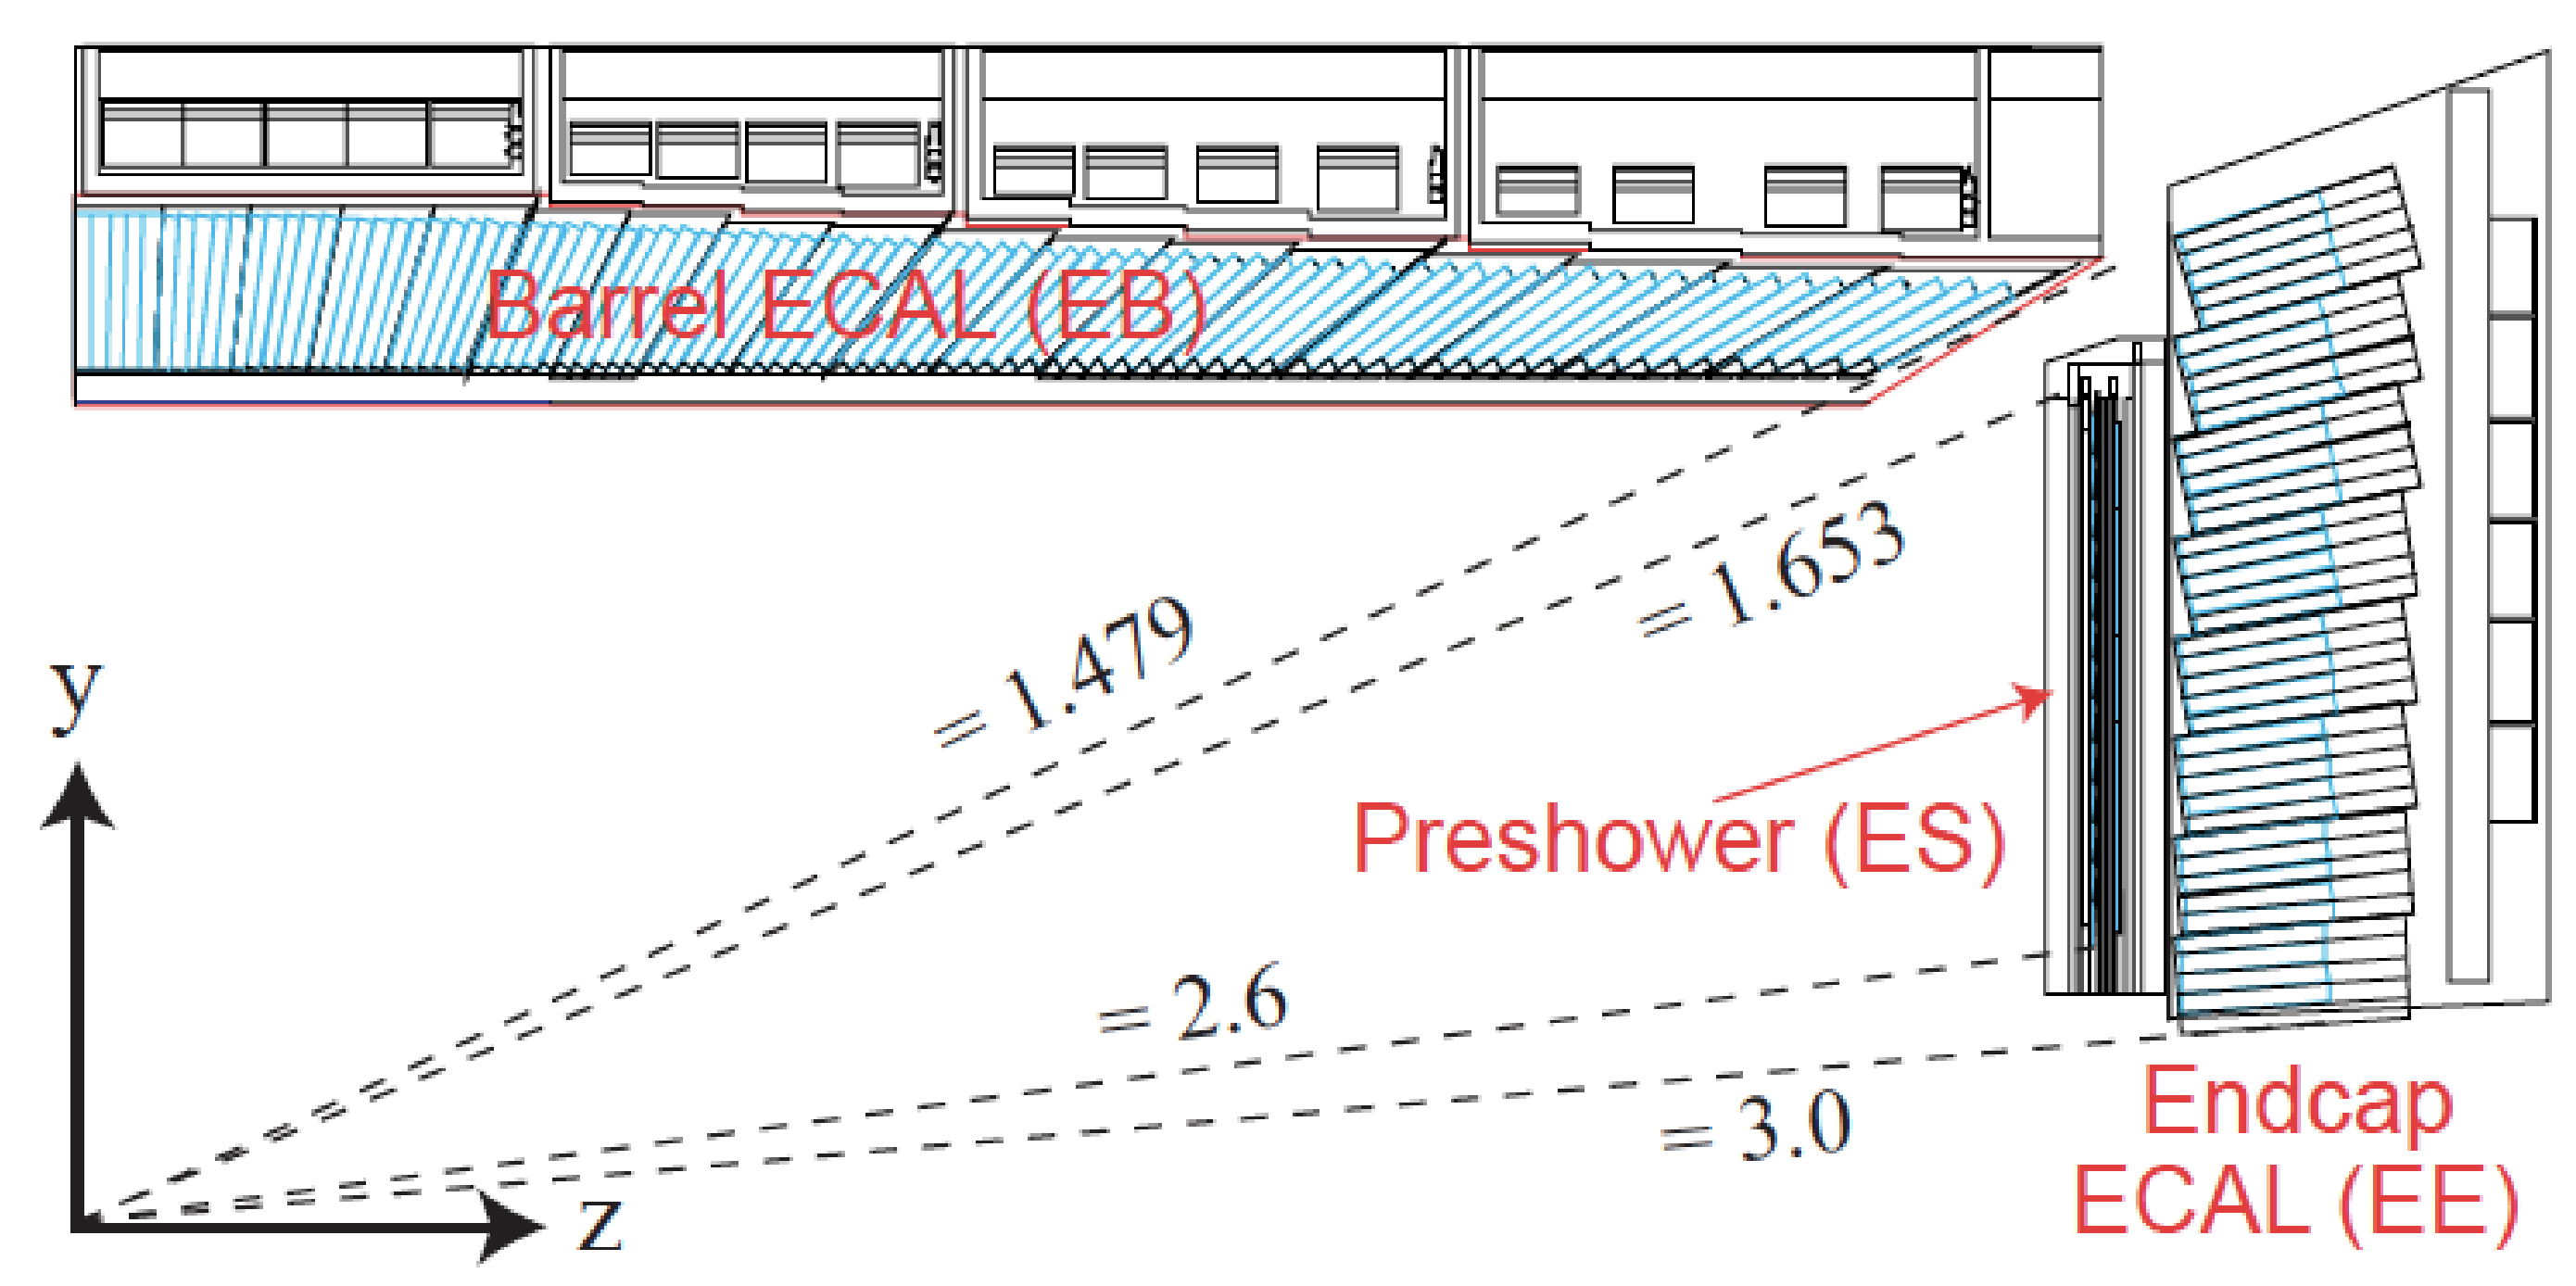
\includegraphics[width=0.5\textwidth]{figures_and_tables/experimental_setup/cms_ecal.png}
    \caption{Longitudinal section view of the ECAL and its components. Source:~\cite{Chatrchyan:2008zzk}.}
    \label{cms_ecal}
\end{figure}

When a electron (or photon) enters the high density region of the lead tungstate crystals (8.3 $g/cm^3$), it initiates a cascade effect of pair production and photon emission via bremsstrahlung. The intensity of light produce is proportional to the energy of the particle adsorbed. With radiation length~\footnote{Distance an electron or a photon travels
until its energy is reduced by a factor of $1/e$.} of 0.89 cm and a small Molière radius (2.2 cm) the ECAL was built with compact size and its fine granularity. The preshower, located in front of the endcap ECAL (EE), is used to distinguish from high momentum photons and pair of photons coming from $\pi^0$ decays, highly boosted, in such a way that they would be indistinguishable one from the other. Its first layer is composed by the lead tungstate crystal, followed by silicon strip sensor, that allow to measure the shape of the initiated cascade on the first layer and correlate this with the source of the radiation. 

Each ECAL crystal is isolated by a carbon fiber layer and it is connected to two photodetectors with a gain of 50. Their signal is collected by a ADC (Analog to Digital Converter) which catches the charge from the photodetectors and convert it to a digital signal.

In the barrel section of the ECAL, an energy resolution of about 1\% is achieved for unconverted or late-converting photons that have energies in the range of tens of GeV. The remaining barrel photons have a resolution of about 1.3\% up to a pseudorapidity of $\abs{\eta} = 1$, rising to about 2.5\% at $\abs{\eta} = 1.4$. In the endcaps, the resolution of unconverted or late-converting photons is about 2.5\%, while the remaining endcap photons have a resolution between 3 and 4\%~\cite{CMS:EGM-14-001}. When combining information from the entire detector, the jet energy resolution amounts typically to 15\% at 10\GeV, 8\% at 100\GeV, and 4\% at 1\TeV, to be compared to about 40\%, 12\%, and 5\% obtained when the ECAL and Hadronic Calorimeter (HCAL) alone are used. 

Due to its responsability on photon and electrons identification, the ECAL had a very important role on the HIggs observation, specially concerning its relation with the $\gamma\gamma$ and 4-leptons finals states of the discovery.



